% !TeX root = ../Thesis.tex

%*****************************************
\chapter{Background}\label{ch:relatedwork}
%*****************************************
\glsresetall % Resets all acronyms to not used

We begin by giving an overview of the technologies and methods used and their domains.

\section{Hardware High-Level Synthesis}

Hardware high-level synthesis is the process of automatically translating an abstract high-level description of a circuit's functionality into the actual specification of the hardware needed to realize it.

\subsection{The VTR Project and VPR}

The open-source \gls{VTR} project\cite{vtr8} provides a complete workflow of Verilog-to-Hardware translation for \gls{FPGA} architectures. It is targeted at research rather than production, and as such also includes various visualisation utilities and benchmarks of different sizes.

The workflow consists of three separate subprojects which can be run in series, but also independently: Odin II performing synthesis of a Verilog description to a \gls{BLIF} netlist, the external ABC project developed at UC Berkeley\cite{ABC-web} performing logic optimization, and the \gls{VPR} project generating and analysing the final layout.

As the name implies, \gls{VPR} performs placing and routing of the \gls{BLIF} netlist it receives as input, but also analyses the produced results concerning timing and resource consumption.

\subsubsection{Netlists}

Netlists are a format of describing the logic of an abstract circuit, containing blocks and a list of nets.

Blocks are hardware primitives like \glspl{LUT}, \gls{I/O} pads, or basic logic functions, which usually are units of fixed dimensions connecting to the circuit via terminals acting either as signal sources or sinks. In a Netlist, blocks do not have coordinates yet but are templates of the actual hardware components needed to perform the desired operation.

A Net is the abstraction of wires connecting specific terminals of the blocks referenced by the net. Each net has a single signal source, the output terminal of some block, which it connects to at least one input terminal of another (or possibly the same) block, its sinks.

In conjunction, these describe the full logical signal paths of a circuit, fully defining its logical behaviour.

\gls{BLIF} provides an open standard format for saving and interchanging logic-level circuit descriptions, enabling interaction of tools from different vendors or projects.\cite{blif-web} \gls{VPR} contains a packing tool to translate circuits in \gls{BLIF} format into Netlists, and therefore supports \gls{BLIF} circuits as input.

\subsubsection{Placement}

Placement is the process of assigning physical locations and orientations to the blocks of a Netlist. While on \glspl{FPGA} the orientation of a block is usually limited by the properties of the available resources at each location, the location itself for each block can be chosen rather freely. However, it is the main task of Placement to choose placements intelligently, so that resource consumption is minimized and performance of the resulting physical circuit is maximized.

The blocks need to be connected physically according to the logical connections listen in the Netlist. Therefore, placing connected blocks close to each other reduces both the consumption of limited wiring resources and signal delays, which impose a hard limit on the possible clock frequency of sequential logic.

In \gls{VPR}, the search for an optimal placement is conducted via a classical simulated annealing algorithm. Possible moves are the swapping of a block's position with another free or occupied valid position. The acceptance criterium of a move is the overall reduction of estimated wiring costs, and moves increasing this cost are accepted only with a certain variable probability.

Over a run of the algorithm, the temporary placement converges towards a weighted local minimum of summed up estimated wiring costs and critical path length. Due to the ability to accept worsening moves, the simulated annealing algorithm can escape bad local minima and to generally produce "good" results. However, as it is a heuristic, no guarantees about the quality of the solution are given.

The quality improvement over increased runtime (controlled linearly by setting the number of moves per temperature level) behaves approximately logarithmically, with a tenfold runtime only achieving 10\% improved quality.\cite{vtr8}

It is this property that warrants our assumption that the algorithm can be improved by introducing a substantial increase in runtime in return for substantially more accurate wiring cost estimates.

\subsubsection{Routing}

Once the blocks are placed, they still need to be connected physically. Not only is a straight connection from signal source to sink usually not possible for most nets as different wires need to be electrically isolated from each other and subsequently must not simply cross, but once there are several sinks in a net, finding the ideal connection structure (lowest accumulated wire length) also becomes an np-hard problem\cite{rsmt-complexity}.

While smart placement can already minimize the need for crossing wires, a certain amount usually remains unavoidable on large circuits. On static architectures like \gls{PCB} or Silicon, this is usually compensated by introducing multiple physical layers via which wires can evade. On \glspl{FPGA} however, wires have to be routed through a grid of connection fabric, where each edge consists of a number of parallel wires called channels, which can be freely connected with any adjacent channel at intersection points by configuring a programmable connection matrix.

These limits in available wiring space/resources cause local bottlenecks, which usually require some of the nets to be connected non-ideally to meet global constraints and minimize resource usage. The process of specifying the physical wiring of all nets under global and local constraints is called Routing.

\gls{VPR} uses a greedy heuristic known as "rip-up and re-route" to achieve Routing. This roughly means routing net after net locally optimally using only the currently remaining resources. Once it is not possible at all to route a net because there are no resources left that would connect all the terminals, the algorithm backtracks and un-routes certain nets, freeing their routing resources.\cite{vtr8}

First and foremost, \gls{VPR} minimizes the global number of parallel channels available at each grid edge. This is achieved by imposing a hard limit, trying to route the circuit, and increasing the limit if no valid routing was found. If the circuit was routed successfully, the limit is reduced, until by manner of binary partitioning the minimum channel count is found.

For the local routing of a single net, the Maze-Router\cite{Maze-Router} algorithm is used, again a greedy heuristic, which is however guaranteed to produce results within a certain margin of the optimal solution (a \gls{RSMT}), as it is at least as good as the corresponding \gls{RMST}.\cite{rmst-quality}

\subsection{Wirelength Estimation}

Estimating the wiring cost of a temporary placement is a central part of the \gls{VPR} Placer. The global wiring cost is computed as the sum of the wiring costs of each net.

Here, the wiring cost is defined as the absolute distance of wiring required for each net. As the effects different nets have on each other are not known before routing the circuit, the wiring distance for each net is computed in isolation assuming abundant resources so any two points in the routing grid can be directly and minimally connected. Together with a uniform grid this results in the Manhattan-distance as the cost of the connection between two points.

However, computing the minimal rectilinear tree connecting the source of a net with all its sinks is an np-hard problem in the number of sinks called \gls{RSMT}.\cite{rsmt-complexity} Furthermore, the wiring cost computation is located at the innermost part of the simulated annealing algorithm used for Placement, which makes it highly runtime-critical.

Therefore, computing the \gls{RSMT} is impractical, and instead, a very simple heuristic is used to estimate the wiring cost of individual nets.

\subsubsection{\gls{HPWL}}

\gls{VPR} uses a scaled variant of the \gls{HPWL} metric, which constitutes a very rough but efficient heuristic for approximating the total path length of the \gls{RSMT} of a net.

\gls{HPWL} is defined as half the perimeter of the axis-aligned minimal \gls{BB} of the terminals connected by the net. It is trivially exact for the case of one and two sinks and provides a lower bound to the minimal wiring cost outside this restriction. 

With increasing sink count, however, this heuristic tends to underestimate the real cost. To combat this behaviour, \gls{VPR} weighs \gls{HPWL} with empirically determined factors relative to the terminal count of a net. While this invalidates the lower-bound property, it generally produces substantially better results than pure \gls{HPWL}.

The reason such a simple and possibly inaccurate estimator was chosen is its efficiency: if the \gls{BB} of a net is known, the \gls{HPWL} can be computed in constant time. As the \glspl{BB} of each affected net are updated whenever a block is moved, which is again highly efficient and does not add to the asymptotic complexity of the Placement algorithm (as moves are at the same level of the program loop as computing the wiring cost, and updating all affected \glspl{BB} is less complex than this).

\subsubsection{Other Common Heuristics}

\begin{figure}
	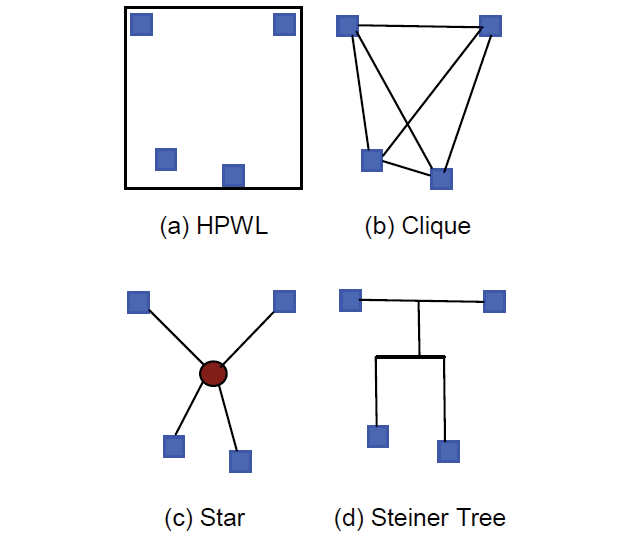
\includegraphics[width=\textwidth]{plots/wirelength-estimation-models.png}
	\caption{Popular wirelength estimation models. (source: \cite{star-plus-paper})}
	\label{fig:wirelength-estimation-models}
\end{figure}

Other popular approaches for in-placement wirelength estimation are the popular star+ model, the clique model, \glspl{RMST}, and \glspl{RSMT}.\cite{star-plus-paper}

While \gls{RSMT} provides the exact minimum possible wirelength, it is an np-hard problem and thus unsuited for in-placement estimation of iterative placers. \gls{RMST} is considerably faster than \gls{RSMT} and overestimates by 50\% at most\cite{rmst-quality}, it still exhibits a high complexity.

The clique model is in quality roughly equivalent as \gls{HPWL}\cite{star-plus-paper} while being more complex and therefore inferior.

The star+ model, on the other hand, can be computed in constant time like \gls{HPWL} but outperforms it measurably. This model estimates the wirelength of a net as the sum of distances from each terminal to the geometric centre of the net. It, therefore, processes more information than the simple \gls{HPWL} model, while still enabling a highly efficient computation.\cite{star-plus-paper}

\section{Neural Networks}

Neural Networks are universal function approximators based on a network of linear combinations followed by non-linear activation functions. They are a group of \gls{ML} algorithms learning their target function by initially making random predictions and improving through the observed error or effect of their predictions.

They usually consist of a layered structure of interconnected artificial neurons, essentially small units, which perform a linear combination of multiple inputs and produce a single output by adjusting that value through a non-linear activation function.

In their basic type, connections between neurons exist only from neurons in one layer to those in the directly adjacent higher layer. This creates a strict feed-forward semantic for prediction, and the weights of the linear combinations can be efficiently updated using a process called backpropagation.

\subsection{Regression}

The application of \glspl{NN} can be divided into Regression Problems and Classification Problems. 

Regression is the task of predicting the value of some variable or multiple variables, usually on a continuous domain, like future temperature prediction based on the weather data of the last few days, or estimating the age of a person depicted in an input image, but also predicting the pixel values of an image, essentially creating a new image.

Classification is the prediction of a discrete class label, e.g. classifying images whether they show cars or not. Classification can be realized as an extension of regression, by first predicting the probability of a certain class, and then introducing a threshold by which to decide if the input is considered part of that class or not.

\subsection{\glspl{CNN}}

\glspl{CNN} are a special class of \glspl{NN}, containing convolutional layers, which essentially implement learnable sliding-window filters over the input tensor. 

With their inherent ability to detect localized structures, \glspl{CNN} perform exceptionally well on image processing, essentially outperforming any other general-purpose image processing algorithm.\cite{dl-vs-cv}\cite{cv-vs-dl}

\subsection{\glspl{RNN}}

\glspl{RNN} contain a feedback loop, breaking the strict one-way forward pass semantic of usual \glspl{NN}. This causes \glspl{RNN} to contain state, enabling them to process sequences of related inputs, creating a single prediction for a sequence of input tensors.

\glspl{RNN} are usually used where the ordering of the input sequences contains relevant information, e.g. temporal sequences of sensor readings.

One important advantage of \glspl{RNN} is their inherent ability to process variable sized inputs without the need for padding or a size limit. While the input tensor dimensions are fixed, the sequence of inputs can have arbitrary length, with each additional tensor adjusting the internal state and thus the prediction.

One of the most popular types of \glspl{RNN} is the \gls{LSTM}\cite{lstm-paper}, a type of \gls{RNN} able to learn long-term dependencies, a task traditional \glspl{RNN} struggle with.\cite{lstm-web}

\subsection{Application in Wirelength Estimation}

In general, \glspl{NN} are able to approximate arbitrarily complex target functions\cite{universial-approx-web} within polynomial asymptotic complexity\cite{NN-complexity-web}. However, in praxis, even simple networks are often sufficient to obtain an estimator achieving very low prediction errors. Not only is the complexity of these estimators lower than their target function, but they also have low runtime in practice, making them faster even for small inputs.

Therefore, we believe \glspl{NN} could be suited as a wiring cost estimator by predicting the wiring cost of the current placement of a net, receiving the coordinates of its terminals as inputs. 

They are expected to produce vastly more accurate estimations than the \gls{HPWL} metric, close to the real optimal wiring cost. Although they will also take substantially more computational effort than \gls{HPWL}, we expect the increased accuracy will help the simulated annealing placement algorithm to correctly judge the effects of its moves, which is an essential part of the algorithm. We hope that this will increase the resulting overall placement quality enough to be able to outperform the unchanged \gls{VPR} on the quality/runtime trade-off, being able to produce higher quality results at same actual runtime, by adjusting the moves per temperature level, at least on part of the runtime domain.

\subsubsection{Target Function}

Training a \gls{NN} using supervised learning requires training examples consisting of sample inputs and their expected prediction value, in our case terminal coordinates and the minimum wiring cost.

However, there are two competing candidates for the minimum wiring cost of a net placement: The \gls{RSMT}, specifying the minimum possible wiring cost, and the length of the wiring tree computed by the Maze-Router algorithm\cite{Maze-Router}, specifying the minimum wiring cost achievable by the \gls{VPR} Router, which might be higher than the \gls{RSMT} cost.

As our goal is to achieve optimal final results for the placed and routed circuit, we have to optimize the Placer to produce outputs optimal for the Router used, so the circuits can be routed efficiently. Therefore, we decided to use the cost computed using the Maze-Router algorithm, optimizing the placement for the routing algorithm present, not for a hypothetical ideal one.

\subsubsection{Related Work}

The deployment of \gls{ML} to \gls{FPGA} hardware synthesis is still rare\cite{routability-estimator}, and we identified only a few publications closely related to our work. 

While there is one paper seemingly covering the same topic as our work, it is hidden behind a paywall, and the accessible abstract does not disclose much useful information.\cite{doi:10.1142/S0218213098000202}

In "Neural network based pre-placement wirelength estimation"\cite{pre-placement-estimation}, Liu et al. deploy \glspl{NN} to estimate wirelengths, however not on individual temporary net placements, but on whole circuits definitions.

Although not related to \glspl{NN}, the contents of the star+ paper incidentally exhibit strong parallels to our work. The authors also develop an in-placement wirelength estimator and evaluate it by implementing it into the \gls{VPR} Placer. The evaluation process deployed by Xu et al. is similar to our own in many aspects but also contains important differences, as detailed in \ref{ch:evaluation}.
